%\section{Results}
%\label{sec:Results}
%% Results should be clear and concise.

The experiment to test the hypothesis that participants in virtual reality (VR) experiments would be more likely to favor data-driven design recommendations for Site Layout Planning (SLP) design was conducted at the Kyushu University campus in Fukuoka, Japan, over a period of 15 days, from June 10 to 25, 2023, during the afternoon hours between 13:00 and 18:00.

A total of 17 participants took part in the experiment, primarily consisting of university students and faculty members. The participants had diverse professional backgrounds, as shown in Figure \ref{fig:ParticipantBackgroundChart}, with over \(50\%\) being students from various faculties, approximately \(20\%\) having a construction background, and \(23.5\%\) reporting previous experience in SLP, as indicated in Figure \ref{fig:YearsExperienceChart}

    %% Participant background chart and years of experience
    \begin{table*}[htb]
        \centering
        \small
        \begin{tabularx}{\textwidth}{X X}
            \centering
            % trim=left 190 down 250 right 150 top5
            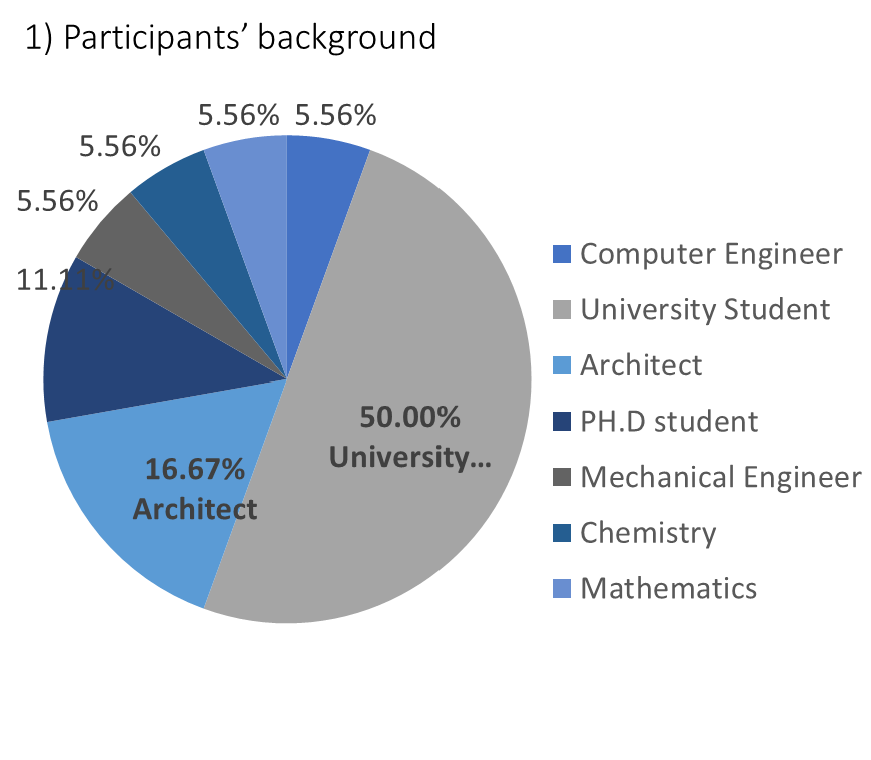
\includegraphics[width=\linewidth, trim=0 50 0 50]{Images/ParticipantBackgroundChart.pdf}
            \captionof{figure}{Professional Background of participants in the experiment for VR in SLP}
            \label{fig:ParticipantBackgroundChart} &
            \centering
            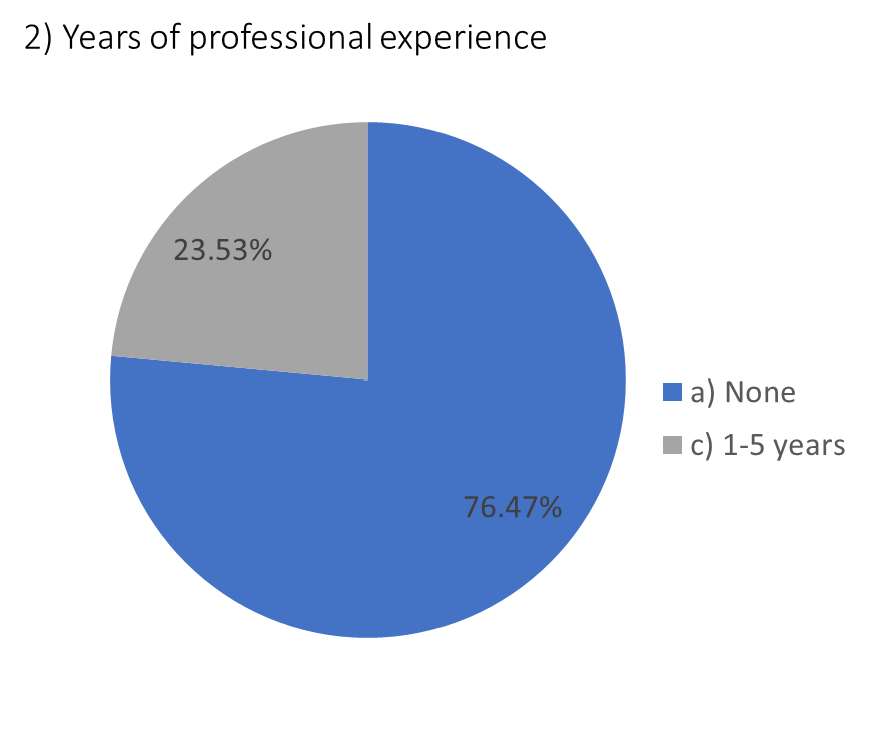
\includegraphics[width=\linewidth, trim=0 50 0 50]{Images/YearsExperienceChart.pdf}
            \captionof{figure}{Years of experience in SLP of participants in the experiment for VR in SLP}
            \label{fig:YearsExperienceChart}
        \end{tabularx}
    \end{table*}

Regarding the first metric, accuracy analysis, most participants completed the SLP task for all three sites, resulting in a total of 39 experiment sessions. For each site, two outcomes were recorded: the position selected during the "screen-based interaction" stage and the "VR interaction" stage. These outcomes were summarized in radial graphs, referred to as "accuracy analysis graphs," as depicted in Figure \ref{fig:Accuracyscattergraph}.

     %% Figure Accuracy graph
        \begin{figure*}[htb]
          \centering
          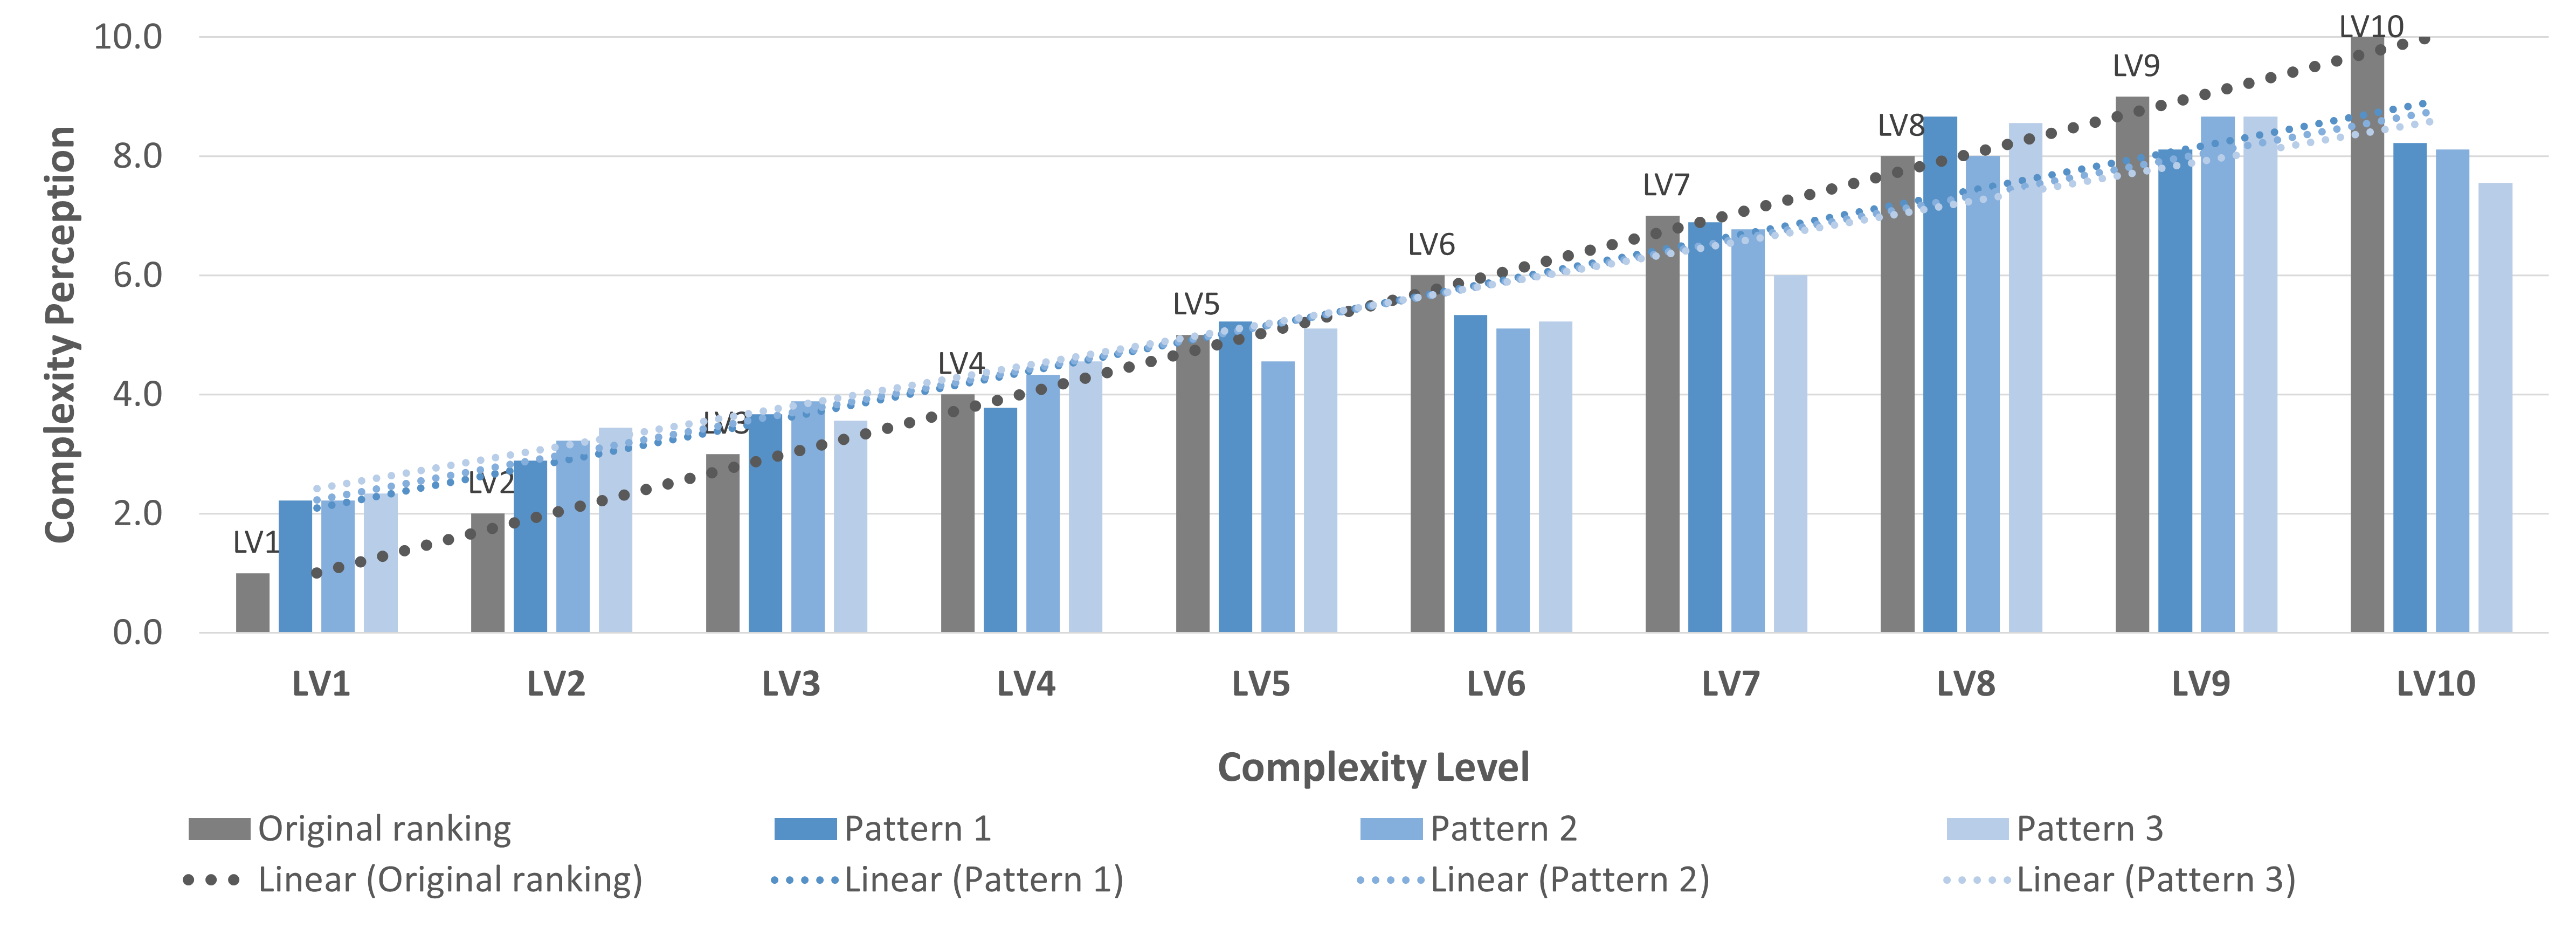
\includegraphics[width= \linewidth, trim=0 0 0 0]{Images/ComplexityPerceptionPerLevel}
          \caption{Complexity perception graph per level of complexity defined for each of the 10 variations generated for each of the three patterns compared to the original ranking. Illustration of the deviation between the complexity perceived by the participants and the original ranking during the screen-based stage of the experiment.}
          \label{fig:ComplexityPerceptionPerLevel}
        \end{figure*}

In these graphs, the center serves as a reference point, representing the top recommendation provided by the optimization system for each specific site. The coordinates of this center point vary for each site, reflecting the distinct optimal locations suggested by the system. On the other hand, the participants' chosen locations are plotted on the graph, precisely indicating the positions they deemed most suitable for the new educational building within the boundaries of the site.

The placement of each participant's chosen location on the graph is based on its actual geographical coordinates, ensuring an accurate representation of their decision-making process. The distance between each participant's chosen location and the center reflects the deviation error from the system's top recommendation, allowing for a clear assessment of how closely participants' choices align with the data-driven optimization results.

Furthermore, the orientation of each chosen location on the graph provides valuable insights into the direction in which participants opted to position the building, allowing for a comprehensive understanding of their decision-making rationale. Overall, these accuracy analysis graphs present an actual representation of the chosen locations on the physical site, capturing both spatial proximity and directional preferences relative to the system's top recommendation.

The purpose of the analysis was to evaluate the reduction in the deviation error between the preferred SLP location recommended by our Multi-objective optimization (MOO) model and the location ultimately chosen by the experiment participants in both the "screen-based" and "VR interaction" stages of the experiment.

By analyzing the accuracy analysis graphs, the contribution of the VR system was determined by examining the vector resultant from the center point (top recommendation) to the participant's chosen location. A reduction in the vector magnitude in the "VR answer" compared to the "screen-based answer" indicated an improvement percentage, while an increase represented a decline. This analysis allowed us to quantify the impact of VR immersion on participants' decision-making accuracy in SLP design.

The accuracy analysis results, depicted in the "Accuracy improvement" bar chart in Figure \ref{fig:ImprovementChart}, showcased varying degrees of improvement among the 39 experiment sessions, with only three cases showing a decline. On average, there was a \(48.3\%\) improvement among the participants.

The accuracy analysis results, illustrated in the "Accuracy improvement" bar chart (Figure \ref{fig:ImprovementChart}), revealed varying degrees of improvement among the 39 experiment sessions, with only three cases showing a decline. On average, there was a significant \(48.3\%\) improvement among the participants.



    % Complexity level chosen Chart
    \begin{figure}[htb]
        \centering
        %trim=100 180 100 120, clip
        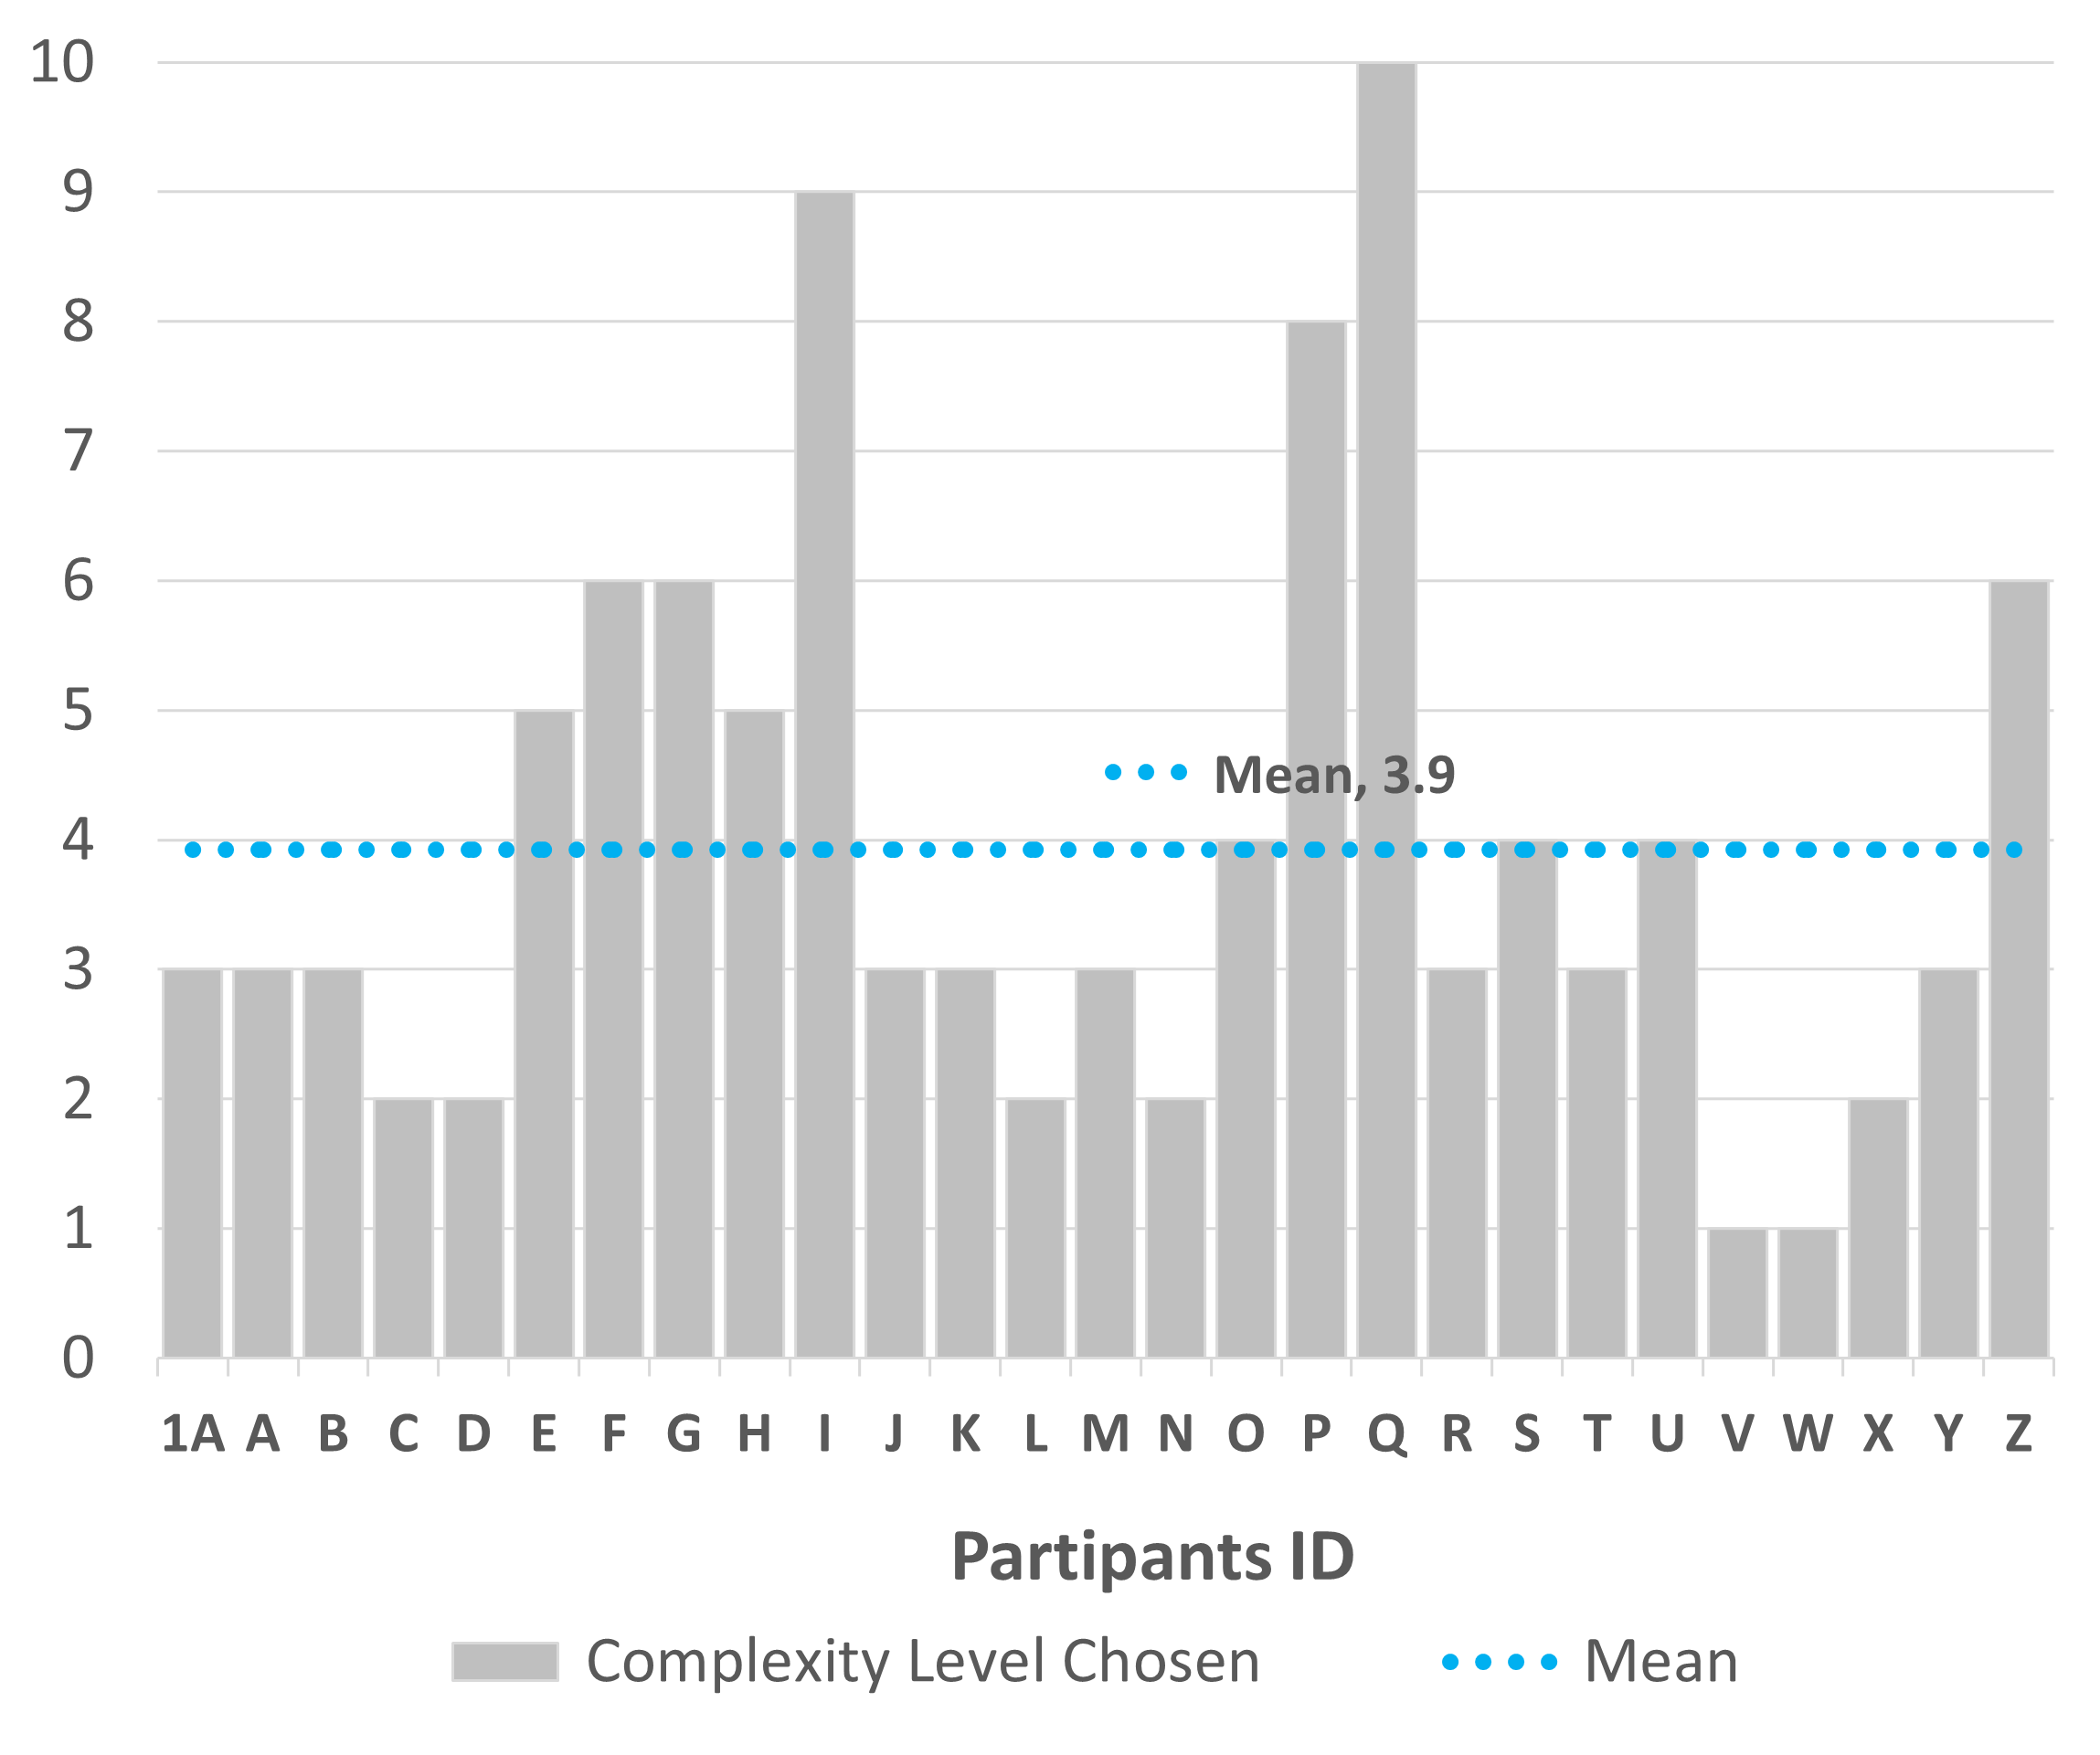
\includegraphics[width=\linewidth]{Images/ComplexityLevelChosenChart}
        \caption{Complexity level chosen among participants during the VR simulation for all three patterns}
        \label{fig:ComplexityLevelChosenChart}
    \end{figure}


    % Complexity perception Chart
    \begin{figure}[htb]
        \centering
        %trim=100 180 100 120, clip
        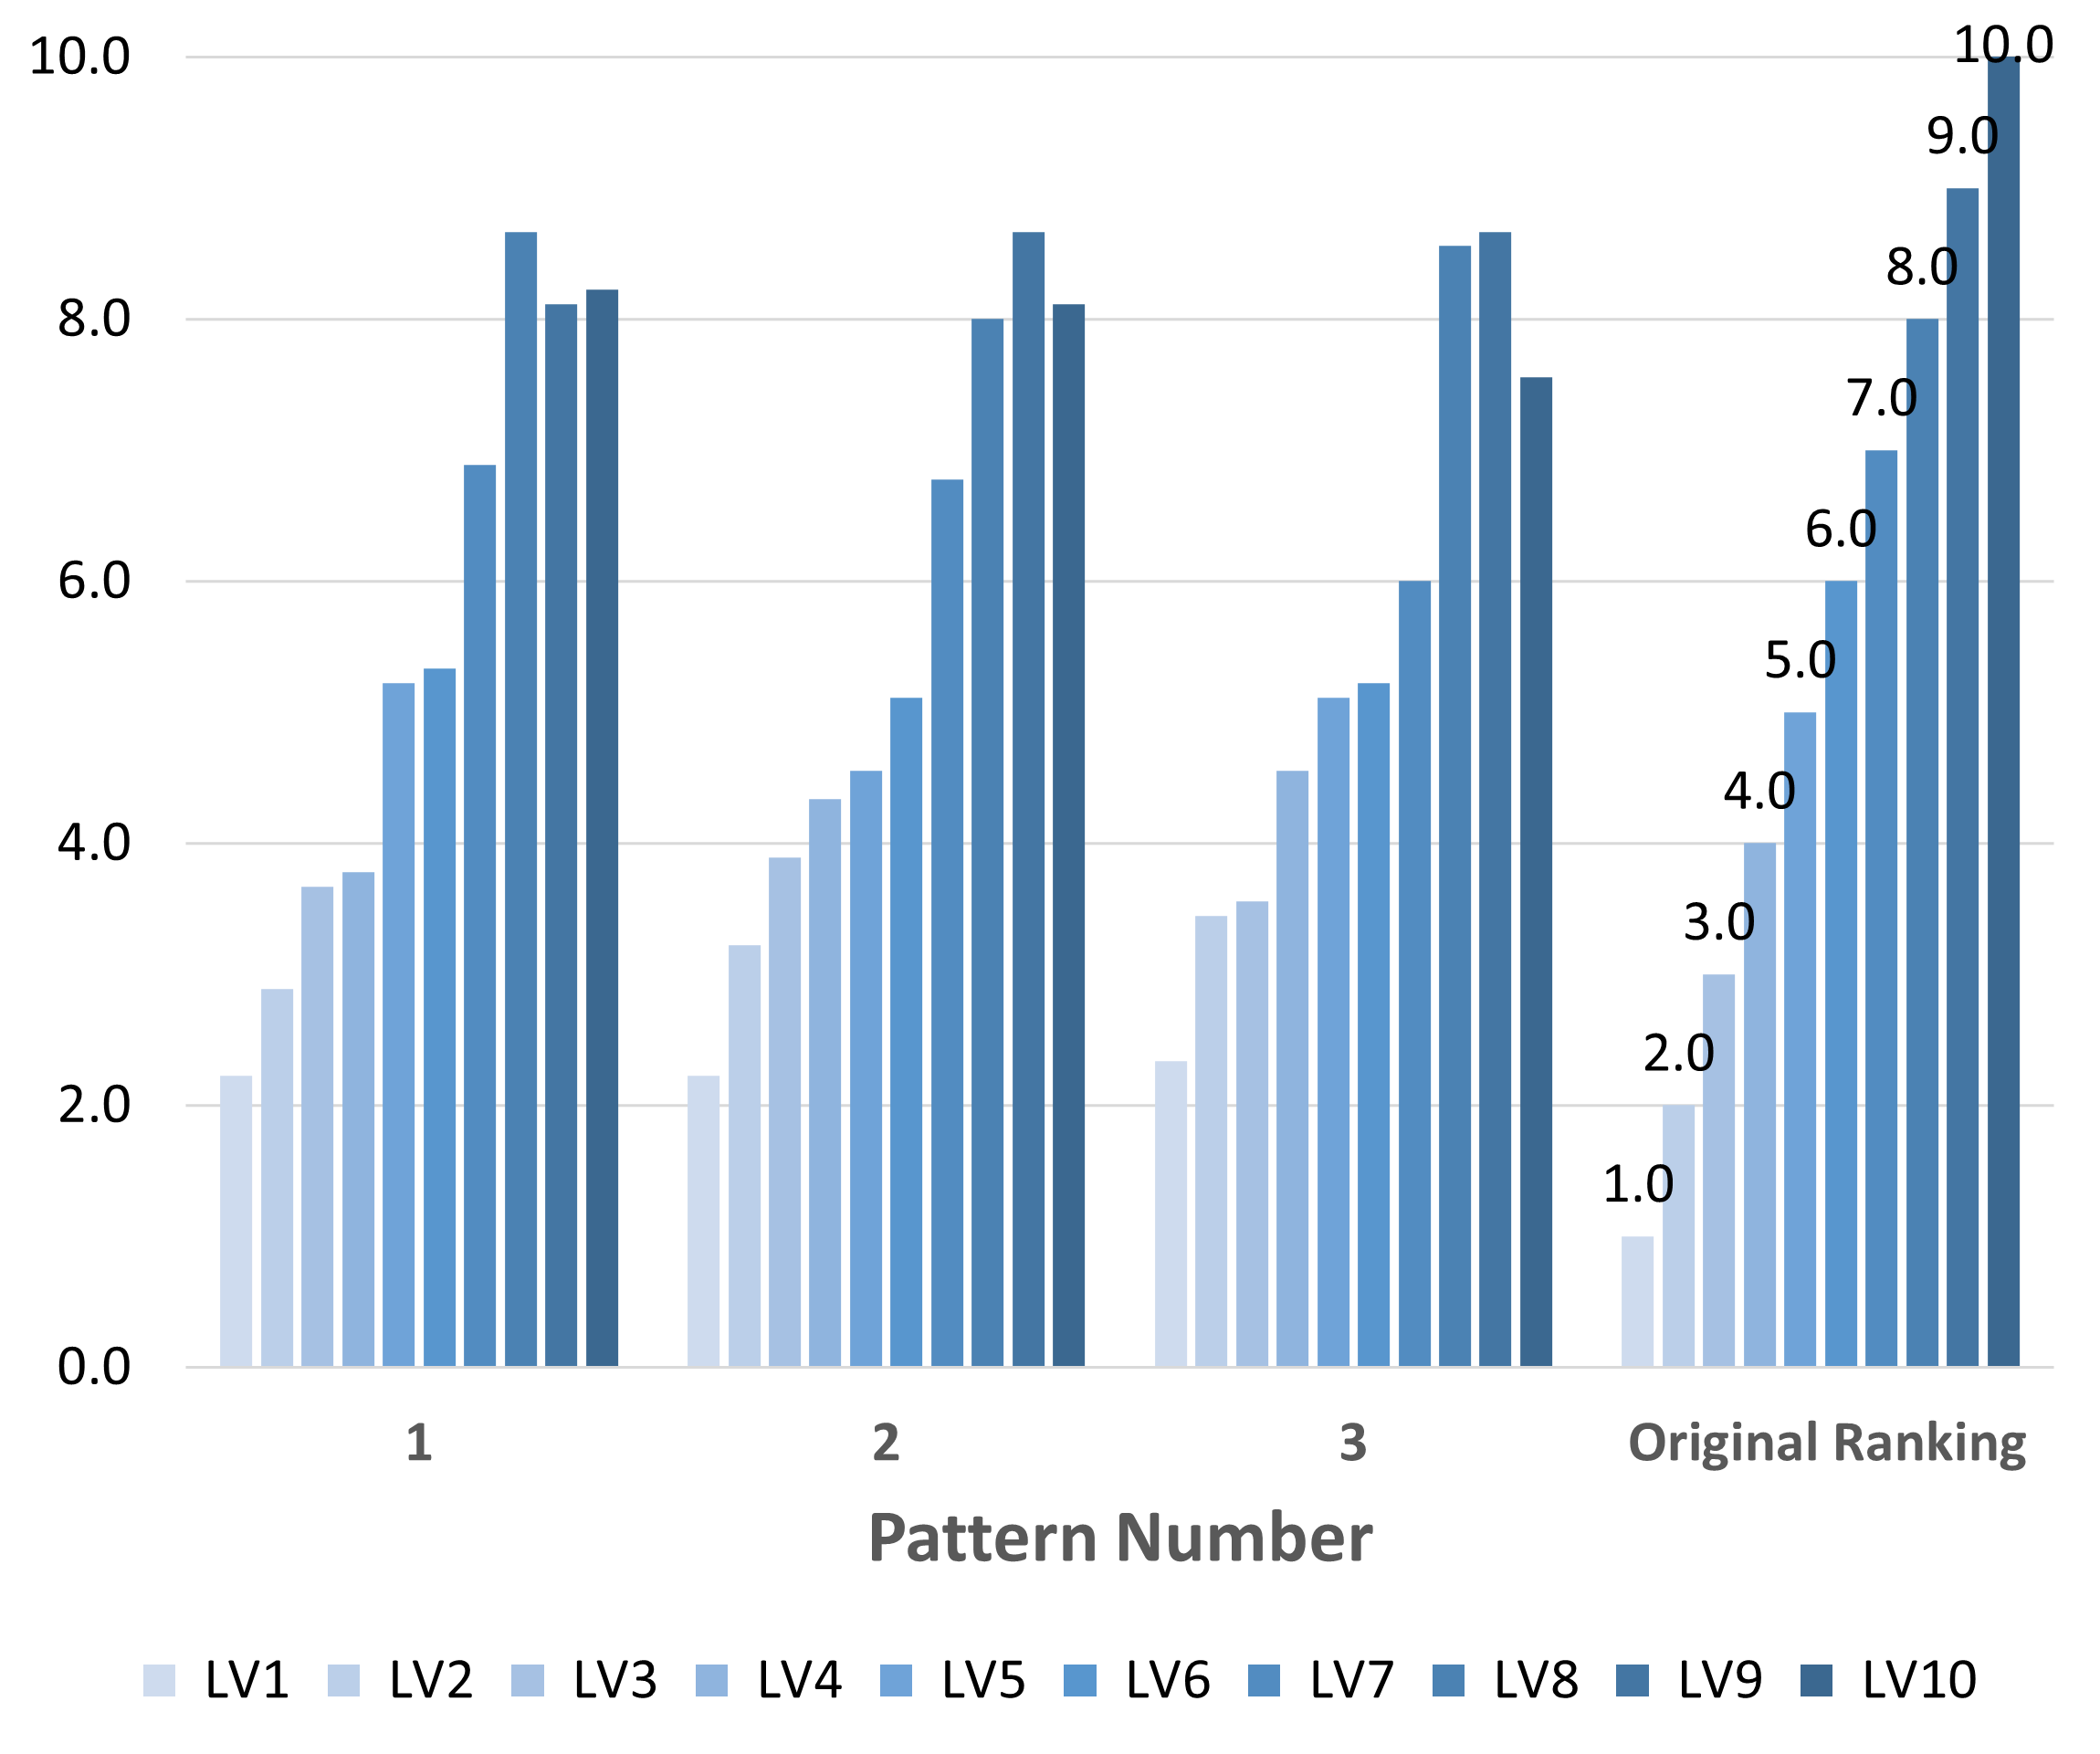
\includegraphics[width=\linewidth]{Images/ComplexityPerceptionChart}
        \caption{Improvement in accuracy among participants with the use of VR simulation compared to the screen-based simulation}
        \label{fig:ComplexityPerceptionChart}
    \end{figure}

The accuracy improvement percentage results exhibited a wide distribution, as indicated by the current standard deviation of \(44.1\%\).
The probability bell graph displayed in Figure \ref{fig:ProbabilityScatterGraph} further illustrated the significant variability in the results, emphasizing the uncertainty in predicting individual data points or outcomes.


% probability preferred complexity level Chart
    \begin{figure}[htb]
        \centering
        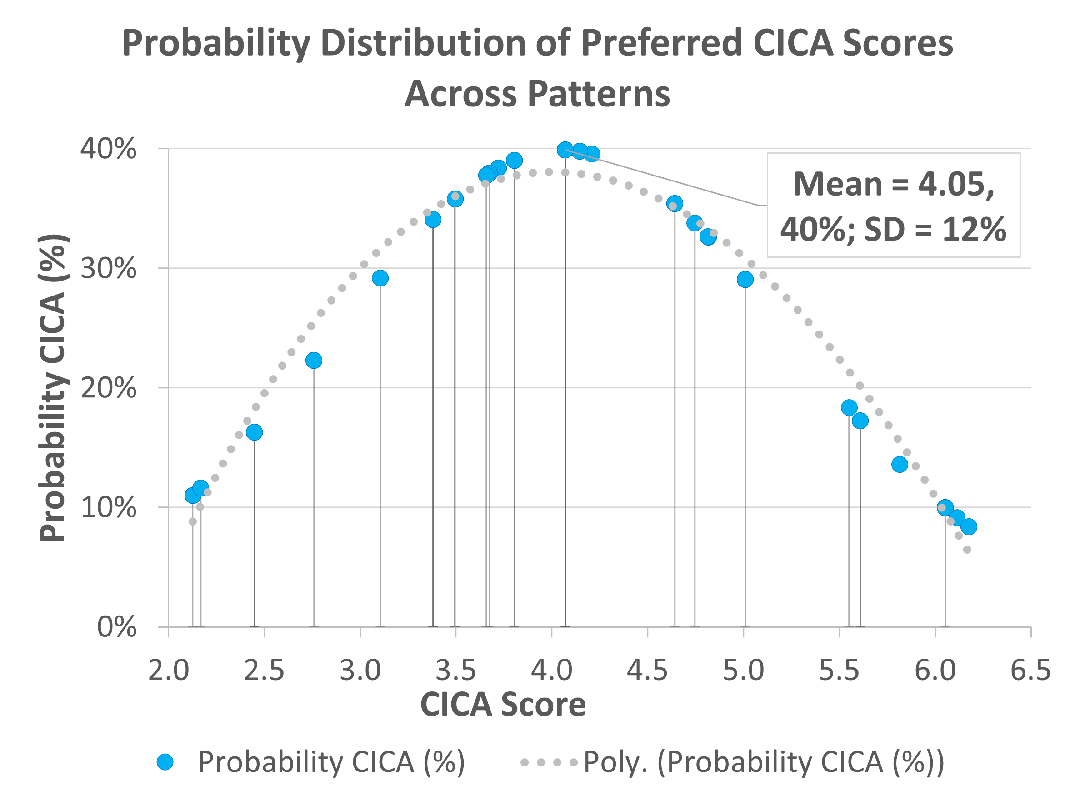
\includegraphics[width=\linewidth]{Images/ProbabilityPreferredComplexitylevel}
        \caption{Probability of preferred complexity level for facade design}
        \label{fig:ProbabilityComplexitylevelChart}
    \end{figure}

Analyzing the average improvement in accuracy per site (Figure \ref{fig:ImprovementPerSite}) revealed a potential correlation between the level of improvement and the complexity of a site's topography.
This finding suggests that VR-based approaches may have a stronger positive impact on decision-making when dealing with more intricate and challenging terrains.

     % Improvement per Site Chart and Performance indicator Weight
    \begin{table*}[htb]
        \centering
        \small
        \begin{tabularx}{\textwidth}{X X}
            \centering
            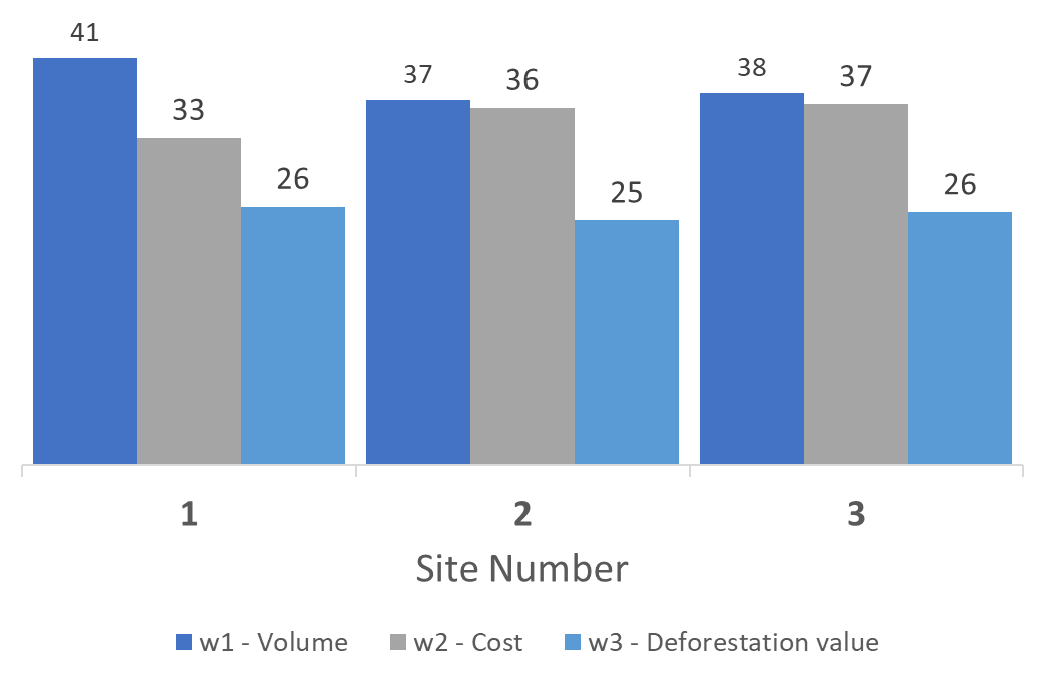
\includegraphics[width=\linewidth, trim=0 0 0 20]{Images/PerformanceIndicatorWeightChart}
            \captionof{figure}{Average of weight distribution when ranking importance of the performance indicators, defined by the participants, per site.}
            \label{fig:PerformanceIndicatorweightChart} &
            \centering
            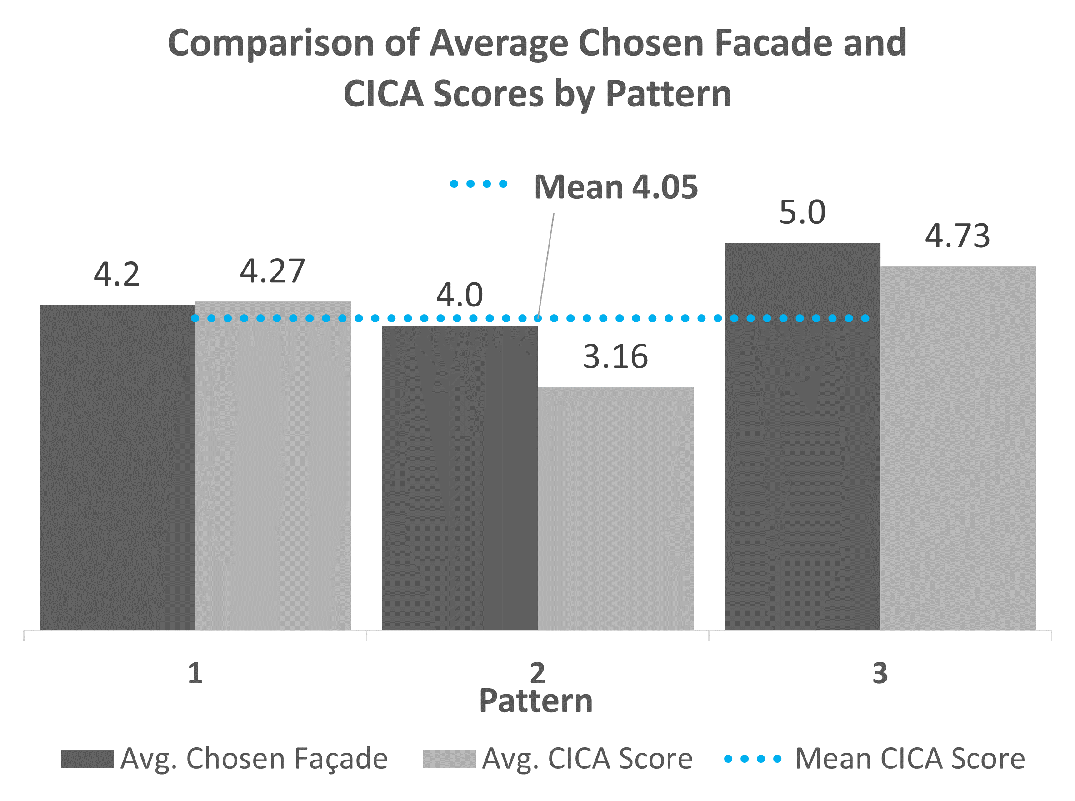
\includegraphics[width=\linewidth, trim=0 0 0 20]{Images/PreferredComplexityLevelPerPattern}
            \captionof{figure}{Average of preferred complexity level per pattern during the VR simulation, with detail of the overall average of the experiment (Mean = \(48.3\%\))}
            \label{fig:ImprovementPerSite}
        \end{tabularx}
    \end{table*}

The survey results provided additional insights into the influence of VR interaction and data-driven optimization for SLP. The ``influence perception'' section of the survey, depicted in Figure\ref{fig:PerceptionSatisfactionSurveyResults}, indicated that the system scored above 5 on a 7-point Likert scale for all questions, suggesting a positive influence of the VR strategy in introducing data-driven recommendations.
This finding aligned with the accuracy improvement percentage results observed in the accuracy analysis (Figure\ref{fig:ImprovementChart}).


  %% Complexity Perception Survey results
    \begin{table*}[htb]
        \centering
        \small
        \begin{tabularx}{\textwidth}{X X}
            \centering
            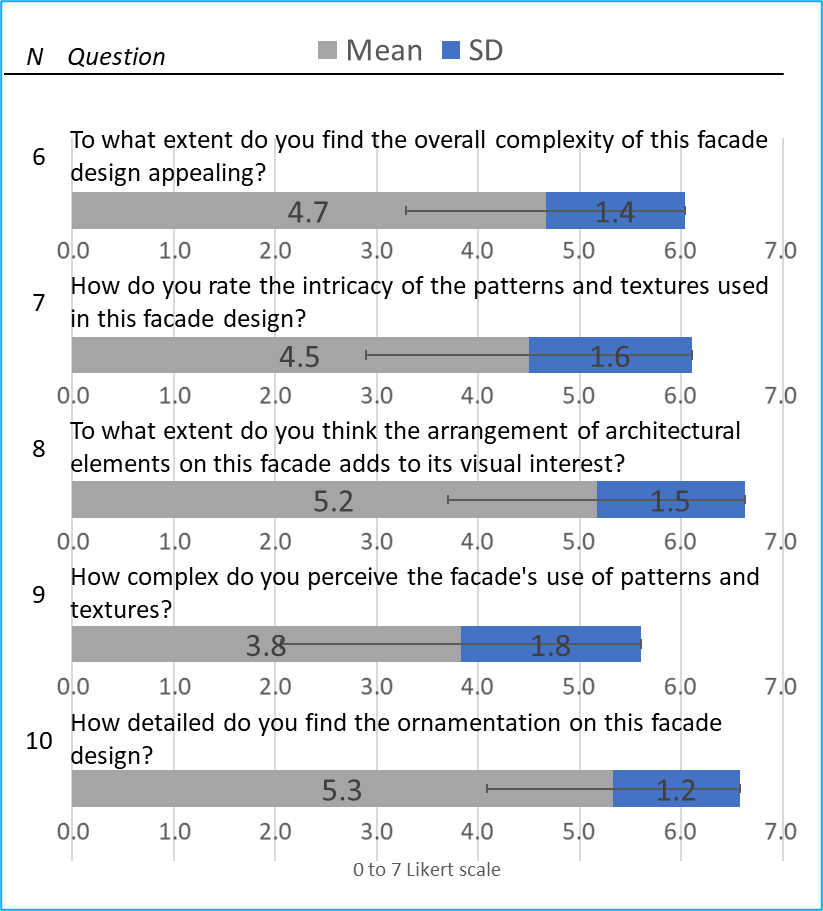
\includegraphics[width=\linewidth]{Images/ComplexitySurveyPart1}
            \captionof{figure}{"User Satisfaction section questions from User Survey of SLP System. \- (n = 17), 1 - strongly disagree, 7 - strongly agree}
            \label{fig:SurveyQuestions6-10} &
            \centering
            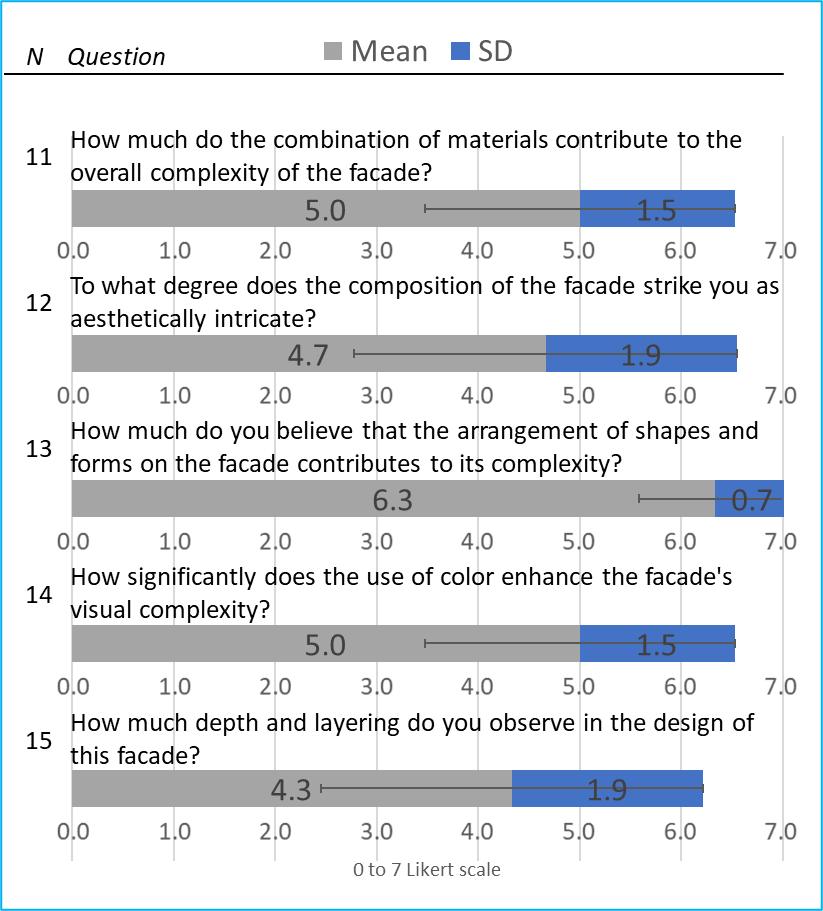
\includegraphics[width=\linewidth]{Images/ComplexitySurveyPart2}
            \captionof{figure}{User-System Influence Perception section" questions. \- (n = 17), 1 - strongly disagree, 7 - strongly agree}
            \label{fig:SurveyQuestions11-15}
        \end{tabularx}
    \end{table*}


During post-experiment interviews, participants were asked for their opinions on the weight distribution used by the optimization model to balance the trade-offs between the three performance indicators.
The initial distribution decided for the system was set at 50, 30, and 20 for the respective indicators (see Table \ref{tab:PerformanceIndicators}).
While most participants maintained a consistent criteria for ranking the indicators, slight deviations from the predetermined weight distribution were observed.
Figure \ref{fig:PerformanceIndicatorweightChart} visually represents the average weight configuration suggested by the participants, demonstrating their individual preferences in adjusting the trade-off weights for each site.

Overall, the results support the initial hypothesis, indicating that VR has the potential to enhance the acceptance of data-driven design recommendations in SLP. However, the "user satisfaction" section of the survey, summarized in Figure \ref{fig:UsabilityChartSurvey}, revealed room for improvement in the user interface and experience, with scores above 4.5 on a 7-point Likert scale.
Notably, the areas of helpfulness and visualization enhancement ranked the lowest, despite initially being considered key advantages of the "VR interaction" system compared to the "screen-based" alternative.
